
\subsection{Pythagorean Identity}
\label{subsec:pythagorean}



\begin{figure}[!h]
    \centering
    \subfloat[Pythagorean Theorem \href{https://socratic.org/questions/58a20042b72cff17846a6feb}{(Source)}]{
  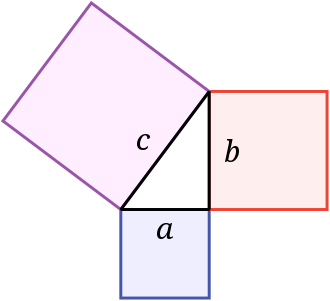
\includegraphics[width=0.3\linewidth]{figures/pythagorean-theorem.png}

  \label{fig:pythagorean-theorem}
}
    \subfloat[Pythagorean Identity \href{https://socratic.org/questions/58a20042b72cff17846a6feb}{(Source)}]{
  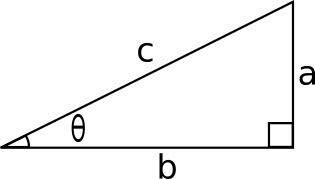
\includegraphics[width=0.3\linewidth]{figures/pythagorean-identity.png}

  \label{fig:pythagorean-identity}
}
  \caption{}
\end{figure}

\begin{tcolorbox}[title={\textbf{\tboxtheorem{\ref*{subsec:pythagorean}} Pythagorean Identity}}]
$\sin^2 \theta + \cos^2 \theta = 1$
\end{tcolorbox}

\begin{proof}
$ $
\begin{enumerate}

\item In \autoref{fig:pythagorean-theorem}, by Pythagorean theorem, $a^2 + b^2 = c^2$.

\item In \autoref{fig:pythagorean-identity}, by definition of sin and cosine,

$\sin\theta = \dfrac{a}{c}, \text{ } \cos\theta = \dfrac{b}{c}$

\item Combining step 1 and 2:

$\sin^2 \theta + \cos^2 \theta = \dfrac{a^2}{c^2} + \dfrac{b^2}{c^2} = \dfrac{a^2 + b^2}{c^2} = 1$


\end{enumerate}
\end{proof}

\subsection{Imaginary Number}
\label{subsec:imaginary}


\begin{tcolorbox}[title={\textbf{\tboxdef{\ref*{subsec:imaginary}} Imaginary Number}}]

\begin{itemize}

\item \boldmath{$i$} is defined to be an imaginary number that has the property: $i^2 =-1$
\item \textbf{Complex Number} is a number that involves imaginary number(s) (e.g., $a = 5.6 + i\cdot4.3)$

\item \textbf{Real Number} is a number that does not involve any imaginary number (e.g., $a = 13.4$)

\item $\overline{a}$ is a \textbf{Conjugate} of $a$ if $a$ and $\overline{a}$ have the same real number part and an opposite-signed imaginary number part

(e.g., $a = 3 + i\cdot3.4$, \text{ } $\overline{a} = 3 - i\cdot3.4$)

\item \textbf{Hermitian Vector} is a vector where the 1st half of its elements is a conjugate of the 2nd half, as the $n$-dimensional vector illustrated below:

$\vec{v} = (v_1, v_2, v_3, \cdots, v_{\frac{n}{2}-1}, v_{\frac{n}{2}}, \overline{v}_{\frac{n}{2}}, \overline{v}_{\frac{n}{2} - 1}, \cdots, \overline{v}_3, \overline{v}_2, \overline{v}_1)$


\end{itemize}
\end{tcolorbox}



\subsection{Euler's Formula}
\label{subsec:euler}




\begin{tcolorbox}[title={\textbf{\tboxdef{\ref*{subsec:euler}} Euler's Formula}}]

$e^{i\theta} = \cos\theta + i\cdot\sin\theta$

\end{tcolorbox}

\begin{figure}[!h]
    \centering
  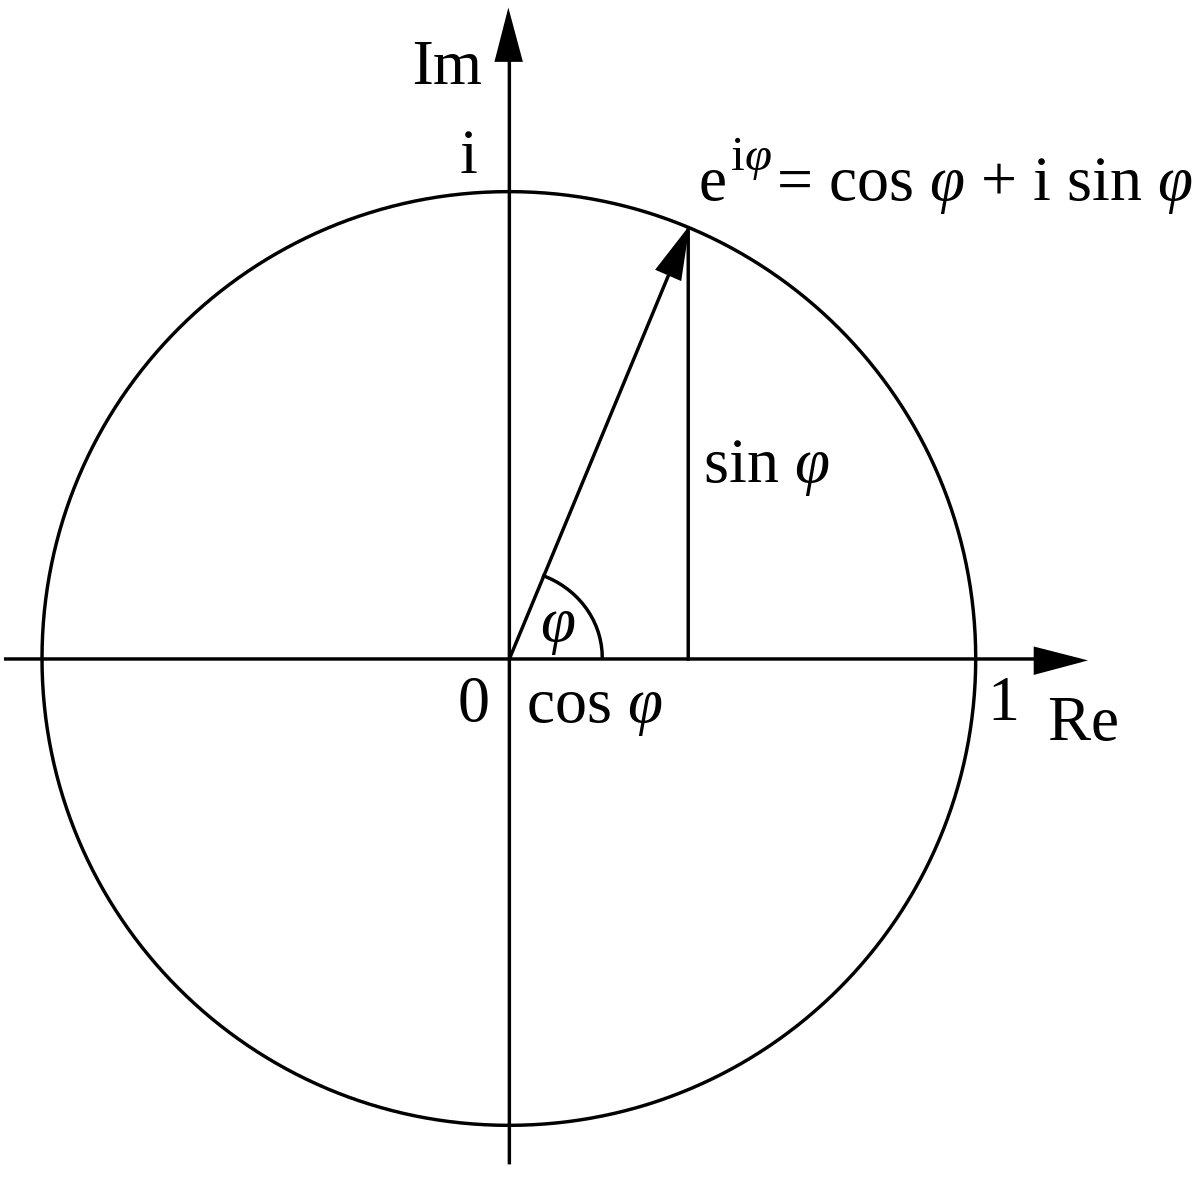
\includegraphics[width=0.4\linewidth]{figures/euler-formula.png}
  \caption{The figure illustrates a circle of Euler's formula in the complex plane \href{https://en.wikipedia.org/wiki/Euler's_formula}{(Source)}}
\end{figure}

The value of $e^{i\theta}$ is represented as a coordinate on a circle in the complex plane in \autoref{fig:complex-plane}, where the $x$-axis encodes the value's real number part and the $y$-axis encodes the value's imaginary number part. Note that as $\theta$ increases, the complex part oscillates between $i$ and $-i$, and the real part oscillates between $1$ and $-1$, with the period of $2\pi$. 


\subsection{Vandermonde Matrix with Roots of Cyclotomic Polynomial over Complex Number}
\label{subsec:vandermonde-euler}

 
 
In this subsection, we will build a Vandermonde matrix (\autoref{subsec:vandermonde}) with the $n$ distinct roots of the $\mu$-th cyclotomic polynomial (where $\mu$ is a power of 2) as follows:



\begin{tcolorbox}[title={\textbf{\tboxtheorem{\ref*{subsec:vandermonde-euler}} Vandermonde Matrix with the Roots of  \text{(power-of-2)}-th Cyclotomic Polynomial over Complex Number}}]

Suppose we have an $n \times n$ (where $n$ is a power of 2) Vandermonde matrix comprised of $n$ distinct roots of the $\mu$-th cyclotomic polynomial (explained in Theorem~\ref*{subsec:cyclotomic-theorem}.1 in \autoref{subsec:cyclotomic-theorem}), where $\mu$ is a power of 2 and $n = \dfrac{\mu}{2}$. In other words, $V = \mathit{Vander}(x_0, x_1, \cdots, x_{n-1})$, where each $x_j = (e^{i\pi/n})^{2j-1}$ for $1 \leq j \leq n$ (i.e., the primitive $\mu$-th roots of unity). Then, the following holds:

$V \cdot V^T = \begin{bmatrix}
0 & \cdots & 0 & 0 & n\\
0 & \cdots & 0 & n & 0\\
0 & \cdots & n & 0 & 0\\
\vdots & \iddots & \vdots & \vdots & \vdots \\
n & 0 & 0 & \cdots & 0\\
\end{bmatrix} = n \cdot I^R_n$

$ $

And $V^{-1} = \dfrac{V^T \cdot I_n^R}{n}$


\end{tcolorbox}

\begin{proof}

$ $

\begin{enumerate}

\item Given $\omega = e^{i\pi/n}$, each $x_j = (\omega)^{2j-1}$. Thus, we can expand as follows:

$V \cdot V^T = \begin{bmatrix}
1 & (\omega) & (\omega)^2 & \cdots & (\omega)^{n-1}\\
1 & (\omega^3) & (\omega^3)^2 & \cdots & (\omega^3)^{n-1}\\
1 & (\omega^5) & (\omega^5)^2 & \cdots & (\omega^5)^{n-1}\\
\vdots & \vdots & \vdots & \ddots & \vdots \\
1 & (\omega^{2n-1}) & (\omega^{2n-1})^2 & \cdots & (\omega^{2n-1})^{n-1}\\
\end{bmatrix} 
\cdot 
\begin{bmatrix}
1 & 1 & 1 & \cdots & 1\\
(\omega) & (\omega^3) & (\omega^5) & \cdots & (\omega^{2n-1})\\
(\omega)^2 & (\omega^3)^2 & (\omega^5)^2 & \cdots & (\omega^{2n-1})^2\\
\vdots & \vdots & \vdots & \ddots & \vdots \\
(\omega)^{n-1} & (\omega^3)^{n-1} & (\omega^5)^{n-1} & \cdots & (\omega^{2n-1})^{n-1}\\
\end{bmatrix} $

$ $


$=
\begin{bmatrix}
\sum\limits_{k=0}^{n-1} \omega^{2k} & \sum\limits_{k=0}^{n-1} \omega^{4k}  & \sum\limits_{k=0}^{n-1} \omega^{6k} & \cdots & \sum\limits_{k=0}^{n-1} \omega^{2nk} \\

\sum\limits_{k=0}^{n-1} \omega^{4k} & \sum\limits_{k=0}^{n-1} \omega^{6k}  & \sum\limits_{k=0}^{n-1} \omega^{8k} & \cdots & \sum\limits_{k=0}^{n-1} \omega^{2k(n+1)} \\

\sum\limits_{k=0}^{n-1} \omega^{6k} & \sum\limits_{k=0}^{n-1} \omega^{8k} & \sum\limits_{k=0}^{n-1} \omega^{10k} & \cdots & \sum\limits_{k=0}^{n-1} \omega^{2k(n+2)} \\

\vdots & \vdots & \vdots & \ddots & \vdots \\
\sum\limits_{k=0}^{n-1} \omega^{2nk} & \sum\limits_{k=0}^{n-1} \omega^{2(n+1)k} & \sum\limits_{k=0}^{n-1} \omega^{2(n+2)k} & \cdots & \sum\limits_{k=0}^{n-1} \omega^{2(n+n-1)k} \\

\end{bmatrix}$

$ $

\item The $V \cdot V^T$ matrix's anti-diagonal elements are $\sum\limits_{k=0}^{n-1} \omega^{2nk}$. We can derive the following:

$\sum\limits_{k=0}^{n-1} \omega^{2nk} = \sum\limits_{k=0}^{n-1} (e^{i\pi/n})^{2nk} = \sum\limits_{k=0}^{n-1}e^{2\pi k i} = \sum\limits_{k=0}^{n-1}(\cos(2\pi k) + i\sin(2\pi k)) = \sum\limits_{k=0}^{n-1} (1 + 0) = n$

This means that the The $V \cdot V^T$ matrix's anti-diagonal elements are $n$. 

$ $

\item Next, we will prove that the $V \cdot V^T$ matrix has 0 for all positions except for the anti-diagonal ones. In other words, we will prove the following: 

$\sum\limits_{k=0}^{n-1} \omega^{2k} = \sum\limits_{k=0}^{n-1} \omega^{4k} = \sum\limits_{k=0}^{n-1} \omega^{6k} = \gap{$\cdots$} = \sum\limits_{k=0}^{n-1} \omega^{2(n-1)k} = \sum\limits_{k=0}^{n-1} \omega^{2(n+1)k} = \gap{$\cdots$} = \sum\limits_{k=0}^{n-1} \omega^{2(2n-1)k} = 0$

For this proof, we will leverage the Geometric Sum formula $\sum\limits_{i=0}^{n-1}x^i = \dfrac{x^n - 1}{x - 1}$:

\begin{tcolorbox}[title={\textbf{\tboxtheorem{\ref*{subsec:vandermonde-euler}.1} Geometric Sum Formula}}]

Let the geometric sum $S_n = 1 + x + x^2 + \cdots + x^{n - 1}$

Then, $x \cdot S_n = x + x^2 + x^3 + \cdots + x^{n}$

$x \cdot S_n - S_n = (x + x^2 + x^3 + \cdots + x^{n}) - (1 + x + x^2 + \cdots + x^{n - 1}) = x^n - 1$

$S_n\cdot (x - 1) = x^n - 1$

$S_n = \dfrac{x^n - 1}{x - 1}$ \textcolor{red}{ \# with the constraint that $x \neq 1$}

\end{tcolorbox}

Leveraging the Geometric Sum formula $\sum\limits_{i=0}^{n-1}x^i = \dfrac{x^n - 1}{x - 1}$, 

$\sum\limits_{k=0}^{n-1} \omega^{2mk} = \dfrac{(\omega^{2m})^n - 1}{\omega^{2m} - 1} = \dfrac{(\omega^{2n})^{m} - 1}{\omega^{2m} - 1} = \dfrac{1 - 1}{\omega^{2m} - 1} = 0$ for $1 \leq m \leq (2n - 1)$  \textcolor{red}{ \# since $\textsf{Ord}(\omega) = 2n$}

Therefore,

$\sum\limits_{k=0}^{n-1} \omega^{2k} = \sum\limits_{k=0}^{n-1} \omega^{4k} = \sum\limits_{k=0}^{n-1} \omega^{6k} = \gap{$\cdots$} = \sum\limits_{k=0}^{n-1} \omega^{2(n-1)k} = \sum\limits_{k=0}^{n-1} \omega^{2(n+1)k} = \gap{$\cdots$} = \sum\limits_{k=0}^{n-1} \omega^{2(2n-1)k} = 0$

$ $

\item Based on the proof of step 2 and 3, $V \cdot V^T = 
\begin{bmatrix}
0 & \cdots & 0 & 0 & n\\
0 & \cdots & 0 & n & 0\\
0 & \cdots & n & 0 & 0\\
\vdots & \iddots & \vdots & \vdots & \vdots \\
n & 0 & 0 & \cdots & 0\\
\end{bmatrix} = n \cdot I_n^R$

\item Given $V \cdot V^T = n \cdot I_n^R$, 

$V^{-1} \cdot V \cdot V^T = V^{-1} \cdot n \cdot I_n^R$

$V^T = V^{-1} \cdot n \cdot I_n^R$

$V^T \cdot I_n^R = V^{-1} \cdot n \cdot I_n^R  \cdot I_n^R$

$V^T \cdot I_n^R = V^{-1} \cdot n$ \textcolor{red}{\text{ } \# since $I_n^R  \cdot I_n^R = I_n$}

$V^{-1} = \dfrac{V^T \cdot I_n^R}{n}$

\end{enumerate}
\end{proof}

Later in the CKKS scheme (\autoref{sec:ckks}), we will use $V^{-1}$ to encode a complex vector into a real number vector, and $V^T$ to decode a real number vector into a complex vector (\autoref{subsec:ckks-enc-dec}).

$ $

\para{Condition for $\bm \mu$:} It's worthwhile to note that the property $V\cdot V^T = n\cdot I_n^R$ does not hold if $\mu$ (denoting the $\mu$-th cyclotomic polynomial) is not a power of 2. In particular, step 3 of the proof does not hold anymore if $\mu$ is not a power of 2:

$\sum\limits_{k=0}^{n-1} \omega^{2k} \neq \sum\limits_{k=0}^{n-1} \omega^{4k} \neq \sum\limits_{k=0}^{n-1} \omega^{6k} \neq \gap{$\cdots$} \neq \sum\limits_{k=0}^{n-1} \omega^{2(n-1)k} \neq \sum\limits_{k=0}^{n-1} \omega^{2(n+1)k} \neq \gap{$\cdots$} \neq \sum\limits_{k=0}^{n-1} \omega^{2(2n-1)k} \neq 0$



\subsection{Vandermonde Matrix with Roots of a Cyclotomic Polynomial over Integer Ring}
\label{subsec:vandermonde-euler-integer-ring}

Theorem~\ref*{subsec:vandermonde-euler} (in \autoref{subsec:vandermonde-euler}) showed that $V \cdot V^T = n \cdot I^R_n$, where $V$ is the Vandermonde matrix $V = \mathit{Vander}(x_0, x_1, \cdots, x_{n-1})$, where each $x_i$ is the primitive $\mu$-th root of unity over $X \in \mathbb{C}$ (i.e., complex number) and $\mu$ is a power of 2. In this subsection, we will show that the relation $V \cdot V^T = n \cdot I^R_n$ holds even if each $x_i$ is the primitive $\mu$-th root of unity over $X \in \mathbb{Z}_p$ (i.e., integer ring). In particular, we will prove Theorem~\ref*{subsec:vandermonde-euler}: 


\begin{tcolorbox}[title={\textbf{\tboxtheorem{\ref*{subsec:vandermonde-euler-integer-ring}} Vandermonde Matrix with Roots of  \text{(power-of-2)}-th Cyclotomic Polynomial over Integer Ring}}]

The proof takes the same format as that of Theorem~\ref*{subsec:vandermonde-euler} (in \autoref{subsec:vandermonde-euler}). Suppose we have an $n \times n$ (where $n$ is a power of 2) Vandermonde matrix comprised of $n$ distinct roots of the $\mu$-th cyclotomic polynomial over $X \in \mathbb{Z}_p$ (integer ring), where $\mu$ is a power of 2 and $n = \dfrac{\mu}{2}$. In other words, $V = \mathit{Vander}(x_0, x_1, \cdots, x_{n-1})$, where each $x_i$ is the root of $X^n + 1$ (i.e., the primitive $(\mu=2n)$-th roots of unity). Then, the following holds:

$V \cdot V^T = \begin{bmatrix}
0 & \cdots & 0 & 0 & n\\
0 & \cdots & 0 & n & 0\\
0 & \cdots & n & 0 & 0\\
\vdots & \iddots & \vdots & \vdots & \vdots \\
n & 0 & 0 & \cdots & 0\\
\end{bmatrix} = n \cdot I^R_n$

$ $

And $V^{-1} = n^{-1}\cdot V^T \cdot I_n^R$


\end{tcolorbox}
\begin{proof}
$ $
\begin{enumerate}
\item $V \cdot V^T$ is expanded as follows:

$V \cdot V^T = \begin{bmatrix}
1 & (\omega) & (\omega)^2 & \cdots & (\omega)^{n-1}\\
1 & (\omega^3) & (\omega^3)^2 & \cdots & (\omega^3)^{n-1}\\
1 & (\omega^5) & (\omega^5)^2 & \cdots & (\omega^5)^{n-1}\\
\vdots & \vdots & \vdots & \ddots & \vdots \\
1 & (\omega^{2n-1}) & (\omega^{2n-1})^2 & \cdots & (\omega^{2n-1})^{n-1}\\
\end{bmatrix} 
\cdot 
\begin{bmatrix}
1 & 1 & 1 & \cdots & 1\\
(\omega) & (\omega^3) & (\omega^5) & \cdots & (\omega^{2n-1})\\
(\omega)^2 & (\omega^3)^2 & (\omega^5)^2 & \cdots & (\omega^{2n-1})^2\\
\vdots & \vdots & \vdots & \ddots & \vdots \\
(\omega)^{n-1} & (\omega^3)^{n-1} & (\omega^5)^{n-1} & \cdots & (\omega^{2n-1})^{n-1}\\
\end{bmatrix} $

$ $


$=
\begin{bmatrix}
\sum\limits_{k=0}^{n-1} \omega^{2k} & \sum\limits_{k=0}^{n-1} \omega^{4k}  & \sum\limits_{k=0}^{n-1} \omega^{6k} & \cdots & \sum\limits_{k=0}^{n-1} \omega^{2nk} \\

\sum\limits_{k=0}^{n-1} \omega^{4k} & \sum\limits_{k=0}^{n-1} \omega^{6k}  & \sum\limits_{k=0}^{n-1} \omega^{8k} & \cdots & \sum\limits_{k=0}^{n-1} \omega^{2k(n+1)} \\

\sum\limits_{k=0}^{n-1} \omega^{6k} & \sum\limits_{k=0}^{n-1} \omega^{8k} & \sum\limits_{k=0}^{n-1} \omega^{10k} & \cdots & \sum\limits_{k=0}^{n-1} \omega^{2k(n+2)} \\

\vdots & \vdots & \vdots & \ddots & \vdots \\
\sum\limits_{k=0}^{n-1} \omega^{2nk} & \sum\limits_{k=0}^{n-1} \omega^{2(n+1)k} & \sum\limits_{k=0}^{n-1} \omega^{2(n+2)k} & \cdots & \sum\limits_{k=0}^{n-1} \omega^{2(n+n-1)k} \\

\end{bmatrix}$

$ $

, where $\omega$ (i.e., the primitive $(\mu=2n)$-th root of unity) has the order $2n$. 

$ $

\item Note that the $V \cdot V^T$ matrix's anti-diagonal elements are $\sum\limits_{k=0}^{n-1} \omega^{2nk}$. It can be seen that $\omega^{2n} \equiv 1 \bmod p$, because $\textsf{Ord}_p(\omega) = 2n$. Thus, the $V \cdot V^T$ matrix's every anti-diagonal element is $\sum\limits_{k=0}^{n-1} 1 = n$.

$ $

\item Next, we will prove that the $V \cdot V^T$ matrix has $0$ for all other positions than the anti-diagonal ones. In other words, we will prove the following: 

$\sum\limits_{k=0}^{n-1} \omega^{2k} = \sum\limits_{k=0}^{n-1} \omega^{4k} = \sum\limits_{k=0}^{n-1} \omega^{6k} = \gap{$\cdots$} = \sum\limits_{k=0}^{n-1} \omega^{2(n-1)k} = \sum\limits_{k=0}^{n-1} \omega^{2(n+1)k} = \gap{$\cdots$} = \sum\limits_{k=0}^{n-1} \omega^{2(2n-1)k} = 0$

$ $

The above is true, because in the particular case of the $(\mu=2n)$-th cyclotomic polynomial $X^n + 1$ (where $n$ is a power of 2), $\omega^{i} + \omega^{i+\frac{n}{2}} \equiv 0 \bmod p$ for each integer $i$ where $0 \leq i \leq n - 1$. Therefore, in the element $\sum\limits_{k=0}^{n-1} \omega^{2k}$, its one-half terms add with its other-half terms and their final summation becomes $0$. This is the same for all other following elements: 

$\sum\limits_{k=0}^{n-1} \omega^{4k}, \text{ } \sum\limits_{k=0}^{n-1} \omega^{6k}, \text{ } \gap{$\cdots$}, \text{ } \sum\limits_{k=0}^{n-1} \omega^{2(n-1)k}, \text{ } \sum\limits_{k=0}^{n-1} \omega^{2(n+1)k}, \text{ } \gap{$\cdots$}, \text{ } \sum\limits_{k=0}^{n-1} \omega^{2(2n-1)k}$

$ $

\item According to step 1 and 2, the $V \cdot V^T$ matrix has $n$ on its anti-diagonal positions and $0$ for all other positions.

\item Now we will derive the formula for $V^{-1}$. Given $V \cdot V^T = n \cdot I_n^R$, 

$V^{-1} \cdot V \cdot V^T = V^{-1} \cdot n \cdot I_n^R$

$V^T = V^{-1} \cdot n \cdot I_n^R$

$V^T \cdot I_n^R = V^{-1} \cdot n \cdot I_n^R  \cdot I_n^R$

$V^T \cdot I_n^R = V^{-1} \cdot n$ \textcolor{red}{\text{ } \# since $I_n^R  \cdot I_n^R = I_n$}

$ $

Now, there is one caveat: modulo operation does not support direct number division (as explained in \autoref{subsec:modulo-division}). This means that the formula $V^{-1} = \dfrac{V^T \cdot I_n^R}{n}$ in Theorem~\ref*{subsec:vandermonde-euler} (in \autoref{subsec:vandermonde-euler}) is inapplicable in our case, because our modulo $p$ arithmetic does not allow direct division of $V^T \cdot I_n^R$ by $n$. Therefore, we instead multiply $V^T \cdot I_n^R$ by the inverse of $n$ (i.e., $n^{-1}$). We continue as follows:

$V^T \cdot I_n^R = V^{-1} \cdot n$

$V^T \cdot I_n^R \cdot n^{-1}= V^{-1} \cdot n \cdot n^{-1}$

$V^{-1} = n^{-1}\cdot V^T \cdot I_n^R$

\end{enumerate}
\end{proof}

We finally proved that $V\cdot V^T = n \cdot I_n^R$, and $V^{-1} = n^{-1}\cdot V^T \cdot I_n^R$. Later in the BFV scheme (\autoref{sec:bfv}), we will use $V^{-1}$ to encode an integer vector into a vector of polynomial coefficients, and $V^T$ to decode it back to the integer vector (\autoref{subsec:bfv-batch-encoding}).

$ $

\para{Condition for $\bm \mu$:} Like in CKSS, it's worthwhile to note that the property $V\cdot V^T = n\cdot I_n^R$ does not hold if $\mu$ (denoting the $\mu$-th cyclotomic polynomial) is not a power of 2. In particular, step 3 of the proof does not hold anymore if $\mu$ is not a power of 2:

$\sum\limits_{k=0}^{n-1} \omega^{2k} \neq \sum\limits_{k=0}^{n-1} \omega^{4k} \neq \sum\limits_{k=0}^{n-1} \omega^{6k} \neq \gap{$\cdots$} \neq \sum\limits_{k=0}^{n-1} \omega^{2(n-1)k} \neq \sum\limits_{k=0}^{n-1} \omega^{2(n+1)k} \neq \gap{$\cdots$} \neq \sum\limits_{k=0}^{n-1} \omega^{2(2n-1)k} \neq 0$